% !TEX TS-program = lualatex
% ^---- This should always be the first line of any lualatex project

\documentclass{article}

% Provides: A way of showing LaTeX-Code side by side with the output it produces.
% TODO: add copyright notice: https://tex.stackexchange.com/questions/19295/side-by-side-source-and-output-when-documenting-a-style-file
% TODO: check whether this copyright notice is needed?


\usepackage[skins,listings]{tcolorbox}

\newtcblisting{latex-example}[2][]{%
  colframe=red!50!yellow!50!black,
  colback=white,
  coltitle=red!50!yellow!3!white,
  bicolor,colbacklower=red!50!yellow!5!white,
  fonttitle=\sffamily\bfseries,
  sidebyside,text and listing,
  title=#2,#1}

% used for "latex-example"-example
\usepackage{tikz}

% Provides: Common style for computational complexity classes and definitions for the most common ones
% TODO: Add copyright notice to Markus Krötzsch

\hyphenation{Exp-Time} % prevents "Ex-PTime"
\hyphenation{NExp-Time} 

\DeclareMathAlphabet{\mathsc}{OT1}{cmr}{m}{sc}

% Define a common style for complexity classes.
% Also use this for less common classes inside the main document.
\newcommand{\complclass}[1]{\ensuremath{\mathsc{#1}}\xspace}

\newcommand{\ACzero}{\complclass{AC$_0$}}
\newcommand{\LogSpace}{\complclass{L}}
\newcommand{\NLogSpace}{\complclass{NL}}
\newcommand{\PTime}{\complclass{P}}
\newcommand{\NP}{\complclass{NP}}
\newcommand{\coNP}{\complclass{coNP}}
\newcommand{\PH}{\complclass{PH}}
\newcommand{\PSpace}{\complclass{PSpace}}
\newcommand{\NPSpace}{\complclass{NPSpace}}
\newcommand{\ExpTime}{\complclass{ExpTime}}
\newcommand{\NExpTime}{\complclass{NExpTime}}
\newcommand{\ExpSpace}{\complclass{ExpSpace}}
\newcommand{\TwoExpTime}{\complclass{2ExpTime}}
\newcommand{\NTwoExpTime}{\complclass{N2ExpTime}}
\newcommand{\ThreeExpTime}{\complclass{3ExpTime}}
\newcommand{\kExpTime}[1]{\complclass{#1ExpTime}}
\newcommand{\kExpSpace}[1]{\complclass{#1ExpSpace}}

% required by the complexity-classes
% TODO: where to actually put it
\usepackage{xspace}




\begin{document}

% the outer tcblisting is used to display once, how the “latex-example”-environment is used in this document.
\begin{tcblisting}{title=Usage of \texttt{latex-example} (for this document only).}
	\begin{latex-example}[lefthand width=3.5cm]{Test123}
	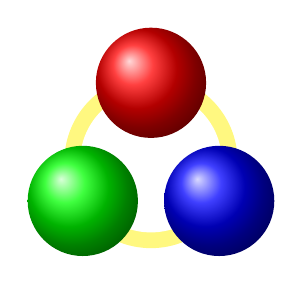
\begin{tikzpicture}
	\path[fill=yellow!50!white] (0,0) circle (11mm);
	\path[fill=white] (0,0) circle (9mm);
	\foreach \w/\c in {90/red,210/green,330/blue}
	{\path[shading=ball,ball color=\c] (\w:1cm) circle (7mm);}
	\end{tikzpicture}
	\end{latex-example}
\end{tcblisting}

\section{Complexity Classes}
\begin{latex-example}{Complexity Classes}
\PTime, \NP and \complclass{APX} are complexity classes.

Clever spacing (\NP-complete),
inline math mode ($\PTime \subseteq \NP$)
and display style
\[
	\PTime \neq \ExpTime
\]
are supported.
\end{latex-example}

\end{document}
